\chapter{Time difference}
\label{ch:timediff}

The ultimate internal background for $\zeronu$ experiments is the $\twonu$ decay of the studied isotope.
Background due to contamination of $^{238}$U decay chain.
When present in the source foils, \Tl\ and \Bi\ can mimic the $\zeronu$ signal by different processes (see Fig.~\ref{fig:internal_contamination}).
For this study, we are focusing on the internal conversion process coming from the contamination of \Tl\ in the source foils.
Regarding the simplified desintegration scheme of the \Tl\ isotope (Fig.~\ref{fig:Tl_scheme}), we see that the $\beta$ desintegration has $51\%$ of probability to fall on the $294$ ps-life time exited level.
To decay to \Pb, the exited isotope has $100\%$ of probability to decay emmiting a $\gamma$ of $2.6$ keV.
In $0.2\%$ of cases, one of the orbital electron can interact with the exited nucleus and decay through internal conversion.
To summarise, decays where a \Tl\ nucleus emmits a $\beta$ particle and then an electron comming from internal conversion of the $2.6$ MeV-$\gamma$ represents $75\%$ of the total $\beta$ decays.
In this case, the internal conversion electron is time-delayed of $294$ ps compared with the $\beta$ particle.
We aim to use this delayed electron to discriminate \Tl\ internal background from signal and other internal backgrounds.

\section{Principle and goal}

\subsection{Internal conversion}
\label{subsec:IC}
Despite its name, internal conversion has nothing to do with the internal probability.
Internal conversion occurs after $\beta$ or $\alpha$ radioactive decays leaving the nucleus exited.
Then a $\gamma$ particle is emitted and transfers its energy to an atomic electron which results in ejection of this electron from the atom.
The emitted electron has an energy corresponding to the energy of previously exited nucleus reduced by the electron binding energy.
After the internal conversion, electrons reorganise.
The hole in internal layer is filled by an electron from an external layer (emitting an X ray).\\
The probability for an atomic electron to be ejected decreases with the initial binding energy.
Thus, electrons from K layers have a higher probability to be converted (see Fig.~\ref{fig:Tl_IC}).

\section{Analysis}
\subsection{Topological cuts}



\subsection{Exponentially modified Gaussian}
\subsection{Results}
\section{Conclusion}


\begin{figure}
  \centering
  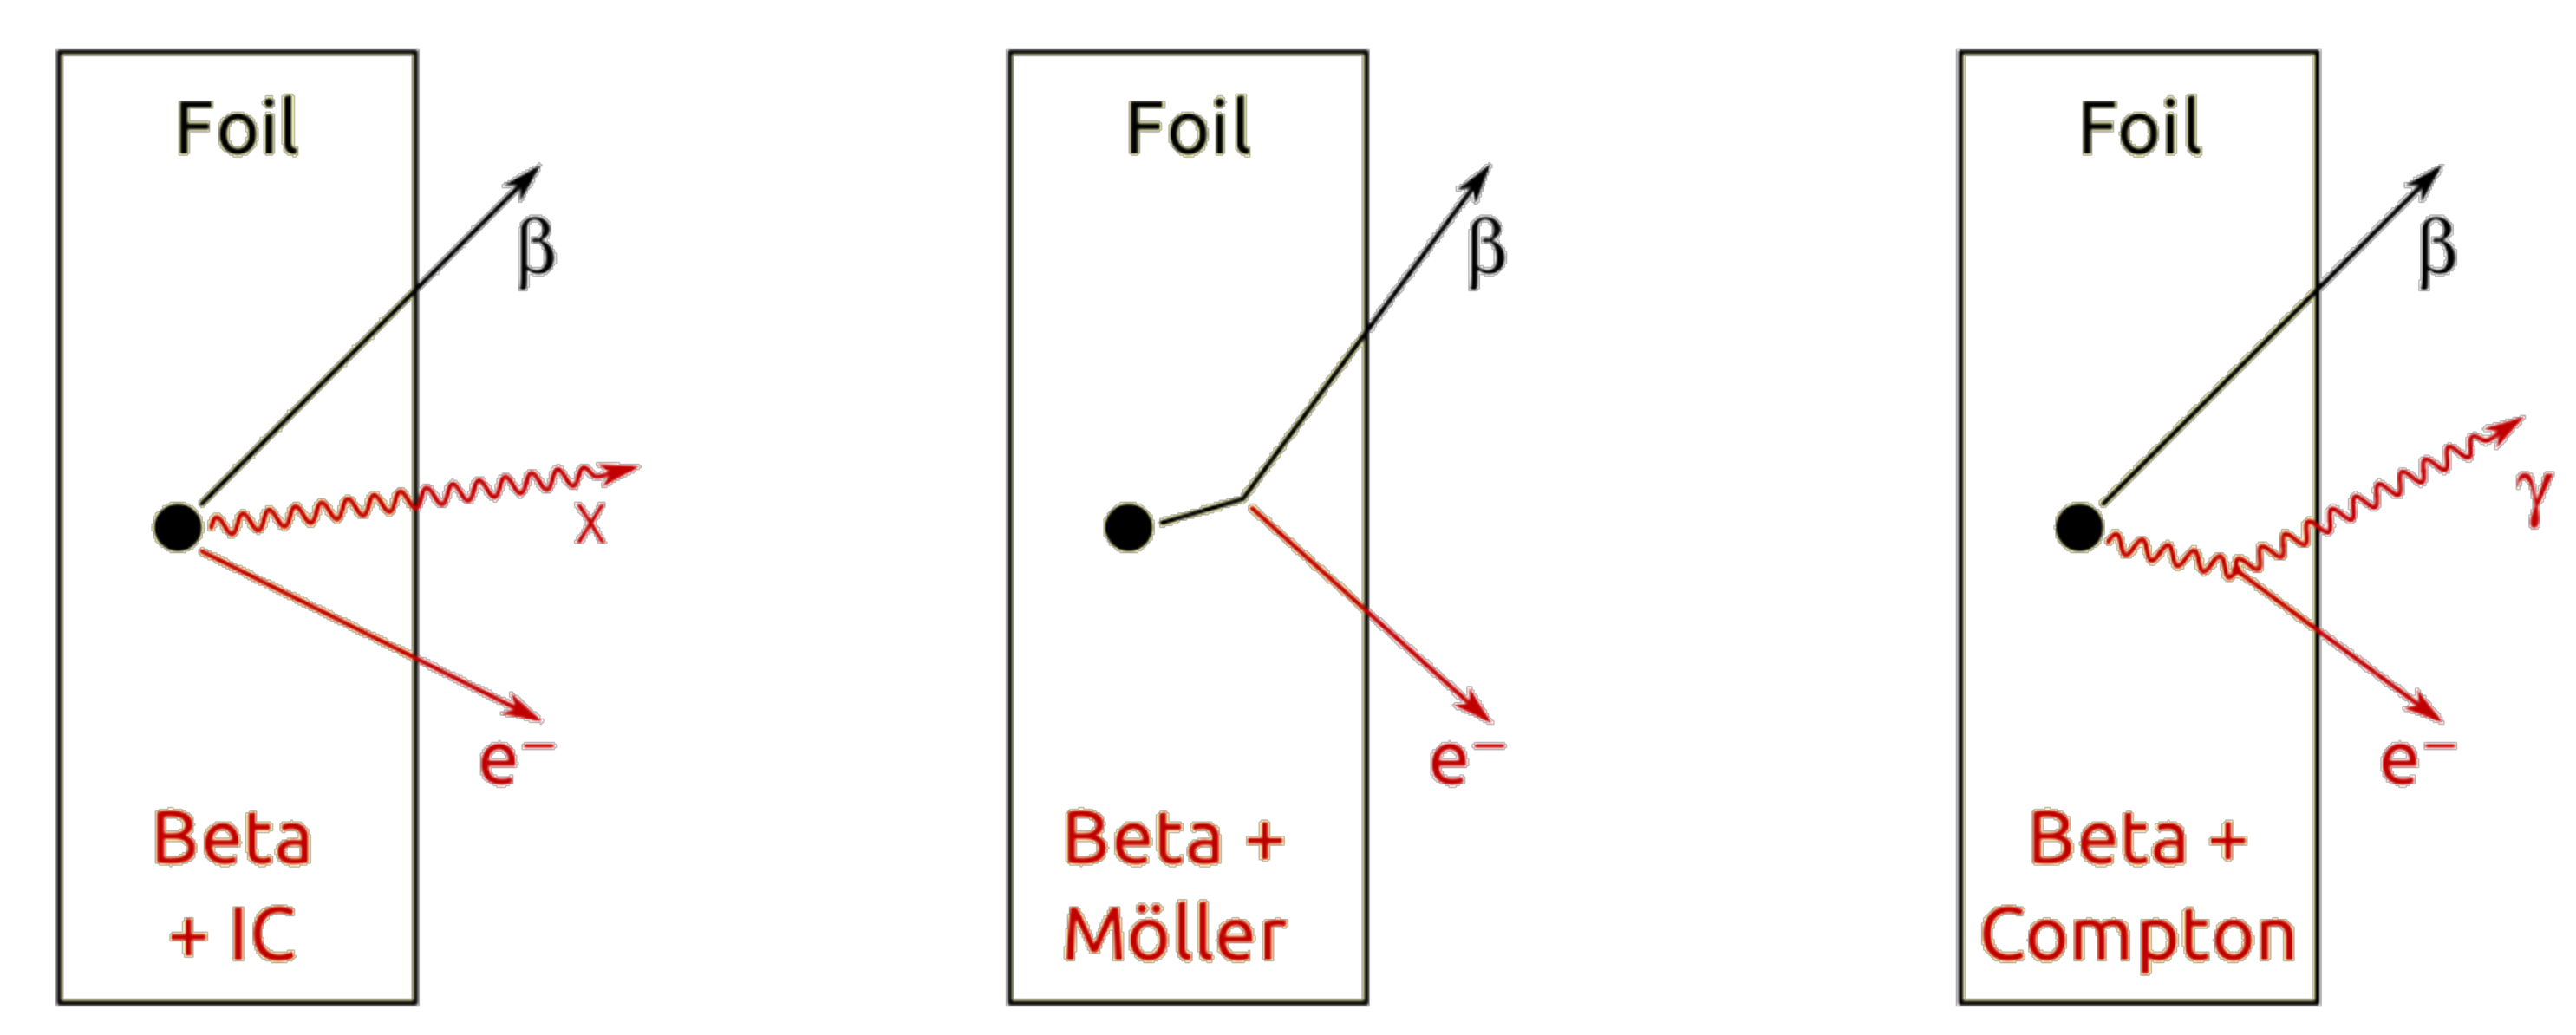
\includegraphics[width=10cm]{timedifference/fig_timediff/internal_contamination.pdf}
  \caption{(a) $\beta$ decay + internal convertion: \Tl\ nucleus performs a $\beta$ decay, then an electron is emitted after internal conversion of photon
    (b) $\beta$ decay + Möller:
    (c) $\beta$ decay + Compton diffusion: \Tl\ nucleus $\beta$ decays to an exited state, then the photon perfoms a Compton diffusion.}
  \label{fig:internal_contamination}
\end{figure}

\begin{figure}
  \centering
  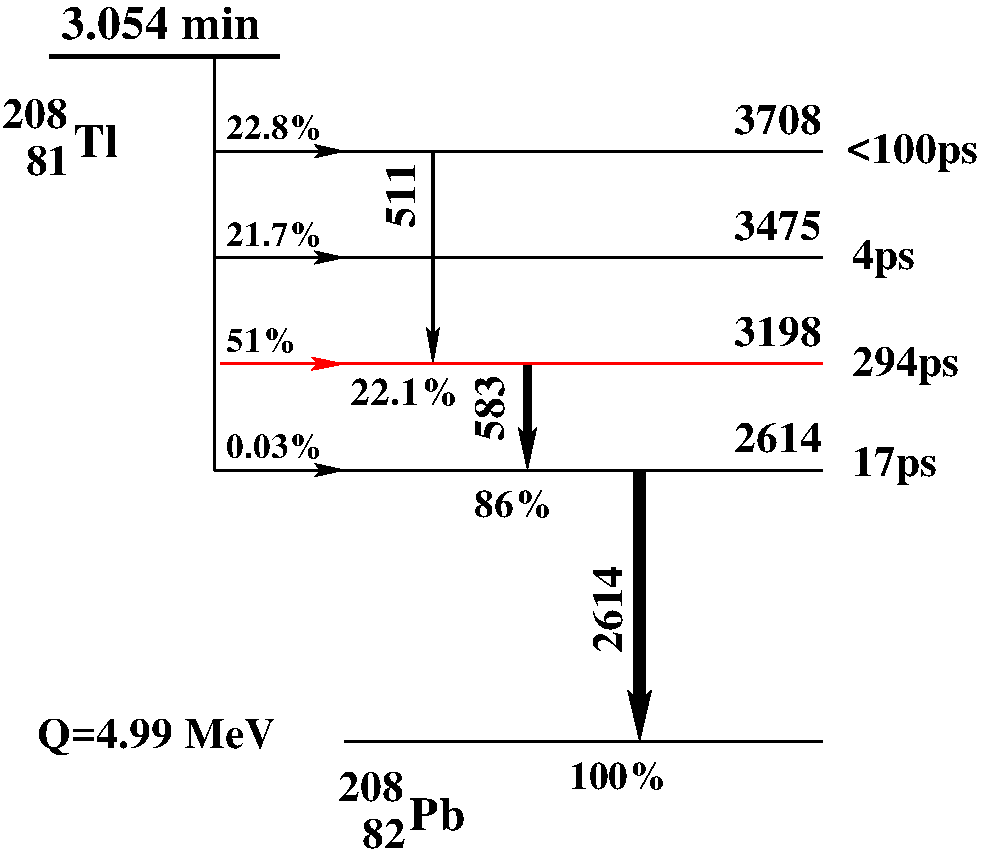
\includegraphics[width=8cm]{timedifference/fig_timediff/Desintegration_Tl.pdf}
  \caption{Simplified desintegration scheme for \Tl\ isotope.
    The level in red has a significant life time of $294$ ps and can be useful in internal backgroung rejection.}
  \label{fig:Tl_scheme}
\end{figure}

\begin{figure}
  \centering
  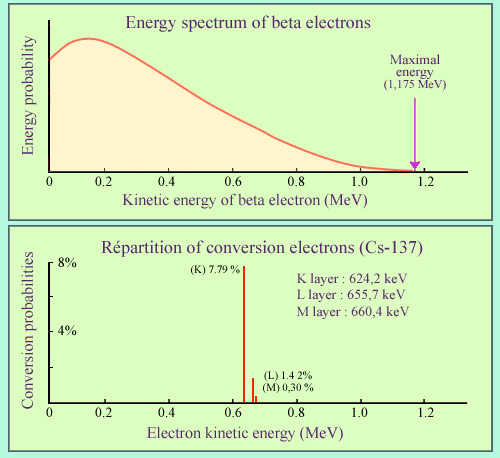
\includegraphics[width=9cm]{timedifference/fig_timediff/SpectreBeta_Cs137.jpg}
  \caption{}
  \label{fig:Tl_IC}
\end{figure}
